\documentclass[sigconf,natbib=true,anonymous]{acmart}
%% RecSys 2026 — Reproducibility Long Paper (8 pages content + unlimited references)
%% Uses ACM sigconf format (two-column layout), double-blind review.
%% Camera-ready: remove 'anonymous' and add author info.

%% Remove ACM-specific elements for cleaner review copy
\settopmatter{printacmref=false}
\renewcommand\footnotetextcopyrightpermission[1]{}
\setcopyright{none}
\acmConference[RecSys'26]{Proceedings of the 20th ACM Conference on Recommender Systems}{September 2026}{TBD}
\acmYear{2026}
\acmDOI{}
\acmISBN{}

\usepackage{booktabs}
\usepackage{multirow}
\usepackage{amsmath,amssymb}
\usepackage{algorithm}
\usepackage{algpseudocode}
\usepackage{graphicx}
\usepackage{subcaption}
\usepackage{siunitx}
\usepackage{xspace}
\usepackage{enumitem}
\usepackage{microtype}
\usepackage{ifthen}
\usepackage{balance}  % Balance columns on last page
\usepackage{hyperref} % Required for \url{} in abstract & body

\newcommand{\model}{\textsc{MV-Align}\xspace}
\newcommand{\base}{\textsc{SASRec}\xspace}
\newcommand{\tfidf}{\textsc{TF-IDF}\xspace}
\newcommand{\llm}{\textsc{LLM}\xspace}
\newcommand{\InfoNCE}{InfoNCE\xspace}

% Circled numbers for figure captions (using textcomp to avoid tikz/amssymb conflict)
\usepackage{pifont}
\newcommand*\circled[1]{\ding{\numexpr171+#1\relax}}

\begin{document}

\title{Multi-View Text Features for Sequential Recommendation:\\
Explicit Cross and Alignment for Reliable Full-Ranking Gains}

% Review version: anonymous authors.
% Camera-ready example:
% \author{First Author}
% \affiliation{\institution{Institution}\country{Country}}
% \email{email@example.com}

\begin{abstract}
% 五句法: 背景-痛点-方案-结果-可复现洞察
Text-feature-enhanced sequential recommenders have attracted growing interest, yet published results are difficult to compare: single-view embeddings, inconsistent evaluation protocols (sampled vs.\ full-ranking), and unreported configuration details hamper reproducibility and may mislead model selection.
%
We present \model, a fully open-sourced, plug-and-play framework that combines multi-view text representations (\tfidf and \llm, with normalization and whitening for decorrelation), explicit ID$\times$Text cross interactions via DCN-V2, and contrastive alignment with cold-start reweighting.
%
The entire pipeline---data preprocessing, feature extraction, training, and evaluation---is released as a single-command reproducible package built on RecBole, enabling one-click replication of every reported result.
%
Under full-ranking evaluation on Amazon Beauty and Toys\&Games, \model achieves HR@10 of \textbf{X.XX}\% and \textbf{X.XX}\% respectively, with notable cold-start gains (HR\_new@10 up to \textbf{X.XX}\%, HR\_few@10 up to \textbf{X.XX}\%).
%% TODO: fill in final numbers once experiments converge.
%
Through controlled ablations with only four tunable knobs, we expose an HR--ranking trade-off and provide two ready-to-use presets (Balanced and Cold/Tail-optimized), offering practitioners actionable guidance on when a frugal \tfidf-only configuration suffices versus when multi-view features pay off.
All code, configurations, and auxiliary analyses are available at \texttt{\url{https://anonymous.4open.science/r/PLACEHOLDER}}.
\end{abstract}

\keywords{Sequential Recommendation, Reproducibility, Text Features, Multi-View Representation, Full-Ranking Evaluation, Open-Source Benchmark}

\maketitle

%% ====================================================================
%% RecSys Reproducibility Long — Target structure (8 pages content)
%%   1. Introduction  (absorbs RQs from former sec_03)
%%   2. Related Work
%%   3. Method         (absorbs Training Protocol from former sec_05)
%%   4. Experimental Setup
%%   5. Results and Analysis  (merges former sec_07 + sec_08)
%%   6. Conclusion
%% ====================================================================

\section{Introduction}

Modern sequential recommenders such as \base~\cite{kang2018sasrec}
provide a strong backbone for modeling user behavior sequences,
yet real-world catalogs are dominated by cold-start and long-tail
items where collaborative signals are sparse. Item text (titles,
descriptions, reviews) offers semantic cues that can improve
generalization, but it also introduces an operational tension:
lightweight features (e.g., \tfidf) are cheap and surprisingly
strong, while \llm-derived embeddings can be richer yet
substantially more expensive in extraction, storage, and serving.

Two practical observations motivate this work. First, once a
strong \tfidf baseline is in place (e.g., +20.0\% HR@10 and
+38.7\% NDCG@10 on Beauty under full ranking), the marginal
gains from adding \llm features can be small and domain-dependent,
making it unclear when multi-view prompting is worth the extra
cost. Second, model selection in industry often relies on fast
sampled evaluation (uniform-100 negatives), but
sampled metrics can disagree with full-ranking metrics and even
mis-rank models~\cite{krichene2020sampledmetrics}; this mismatch
is particularly harmful when improvements concentrate on
cold-start/long-tail strata.

\model addresses this contradiction with a simple
``prepare--interact--align'' recipe (Figure~\ref{fig:cover}):

\textbf{(1) Prepare} (representation level): We normalize
and whiten each text view independently to address three failure
modes---scale mismatch across views, view-to-view correlation,
and cross-view redundancy. Whitening decorrelates multi-view
channels, making subsequent interactions more learnable.

\textbf{(2) Interact} (fusion level): We use an explicit cross
network (DCN-V2) to learn high-order ID$\times$text feature
crosses. While Transformer self-attention models sequence-level
item--item dependencies, it does not explicitly capture
feature-level interactions between ID embeddings and text
embeddings; DCN-V2 fills this gap through element-wise products
gated by learned weight matrices.

\textbf{(3) Align} (objective level): We align each text view
to the collaborative ID embedding space via InfoNCE contrastive
loss. Alignment targets are (text view $\to$ ID space); positive
pairs are (item's text view, item's ID embedding); negatives are
in-batch items. Cold-start reweighting prevents frequent items
from dominating the alignment signal, ensuring that
low-popularity items receive sufficient gradient updates.

Our contributions are threefold.
\begin{itemize}[leftmargin=*,itemsep=1pt]
  \item We propose \model, a deployable plug-in framework for
    \base that supports a frugal \tfidf-only configuration as
    well as stronger multi-view \llm features under a fixed
    embedding budget.
  \item We benchmark on two Amazon domains (Beauty and
    Toys\&Games) with \textbf{full-ranking} evaluation and
    popularity-stratified metrics, and provide systematic
    ablations (whitening, SE-style gating, cross) alongside robustness
    analyses (hyperparameter sensitivity/stability) in the
    appendix.
  \item We go beyond reporting gains by explaining a key
    phenomenon: whitening and explicit cross can improve
    ranking quality (MRR/NDCG) while slightly hurting recall
    (HR), revealing an HR--ranking trade-off that guides when
    to choose lightweight versus stronger configurations.
\end{itemize}
The rest of the paper is organized as follows: we review
related work, introduce \model and the two-phase training
protocol, present full-ranking results and ablations, and
conclude with analyses and takeaways.

\begin{figure*}[t]
\centering
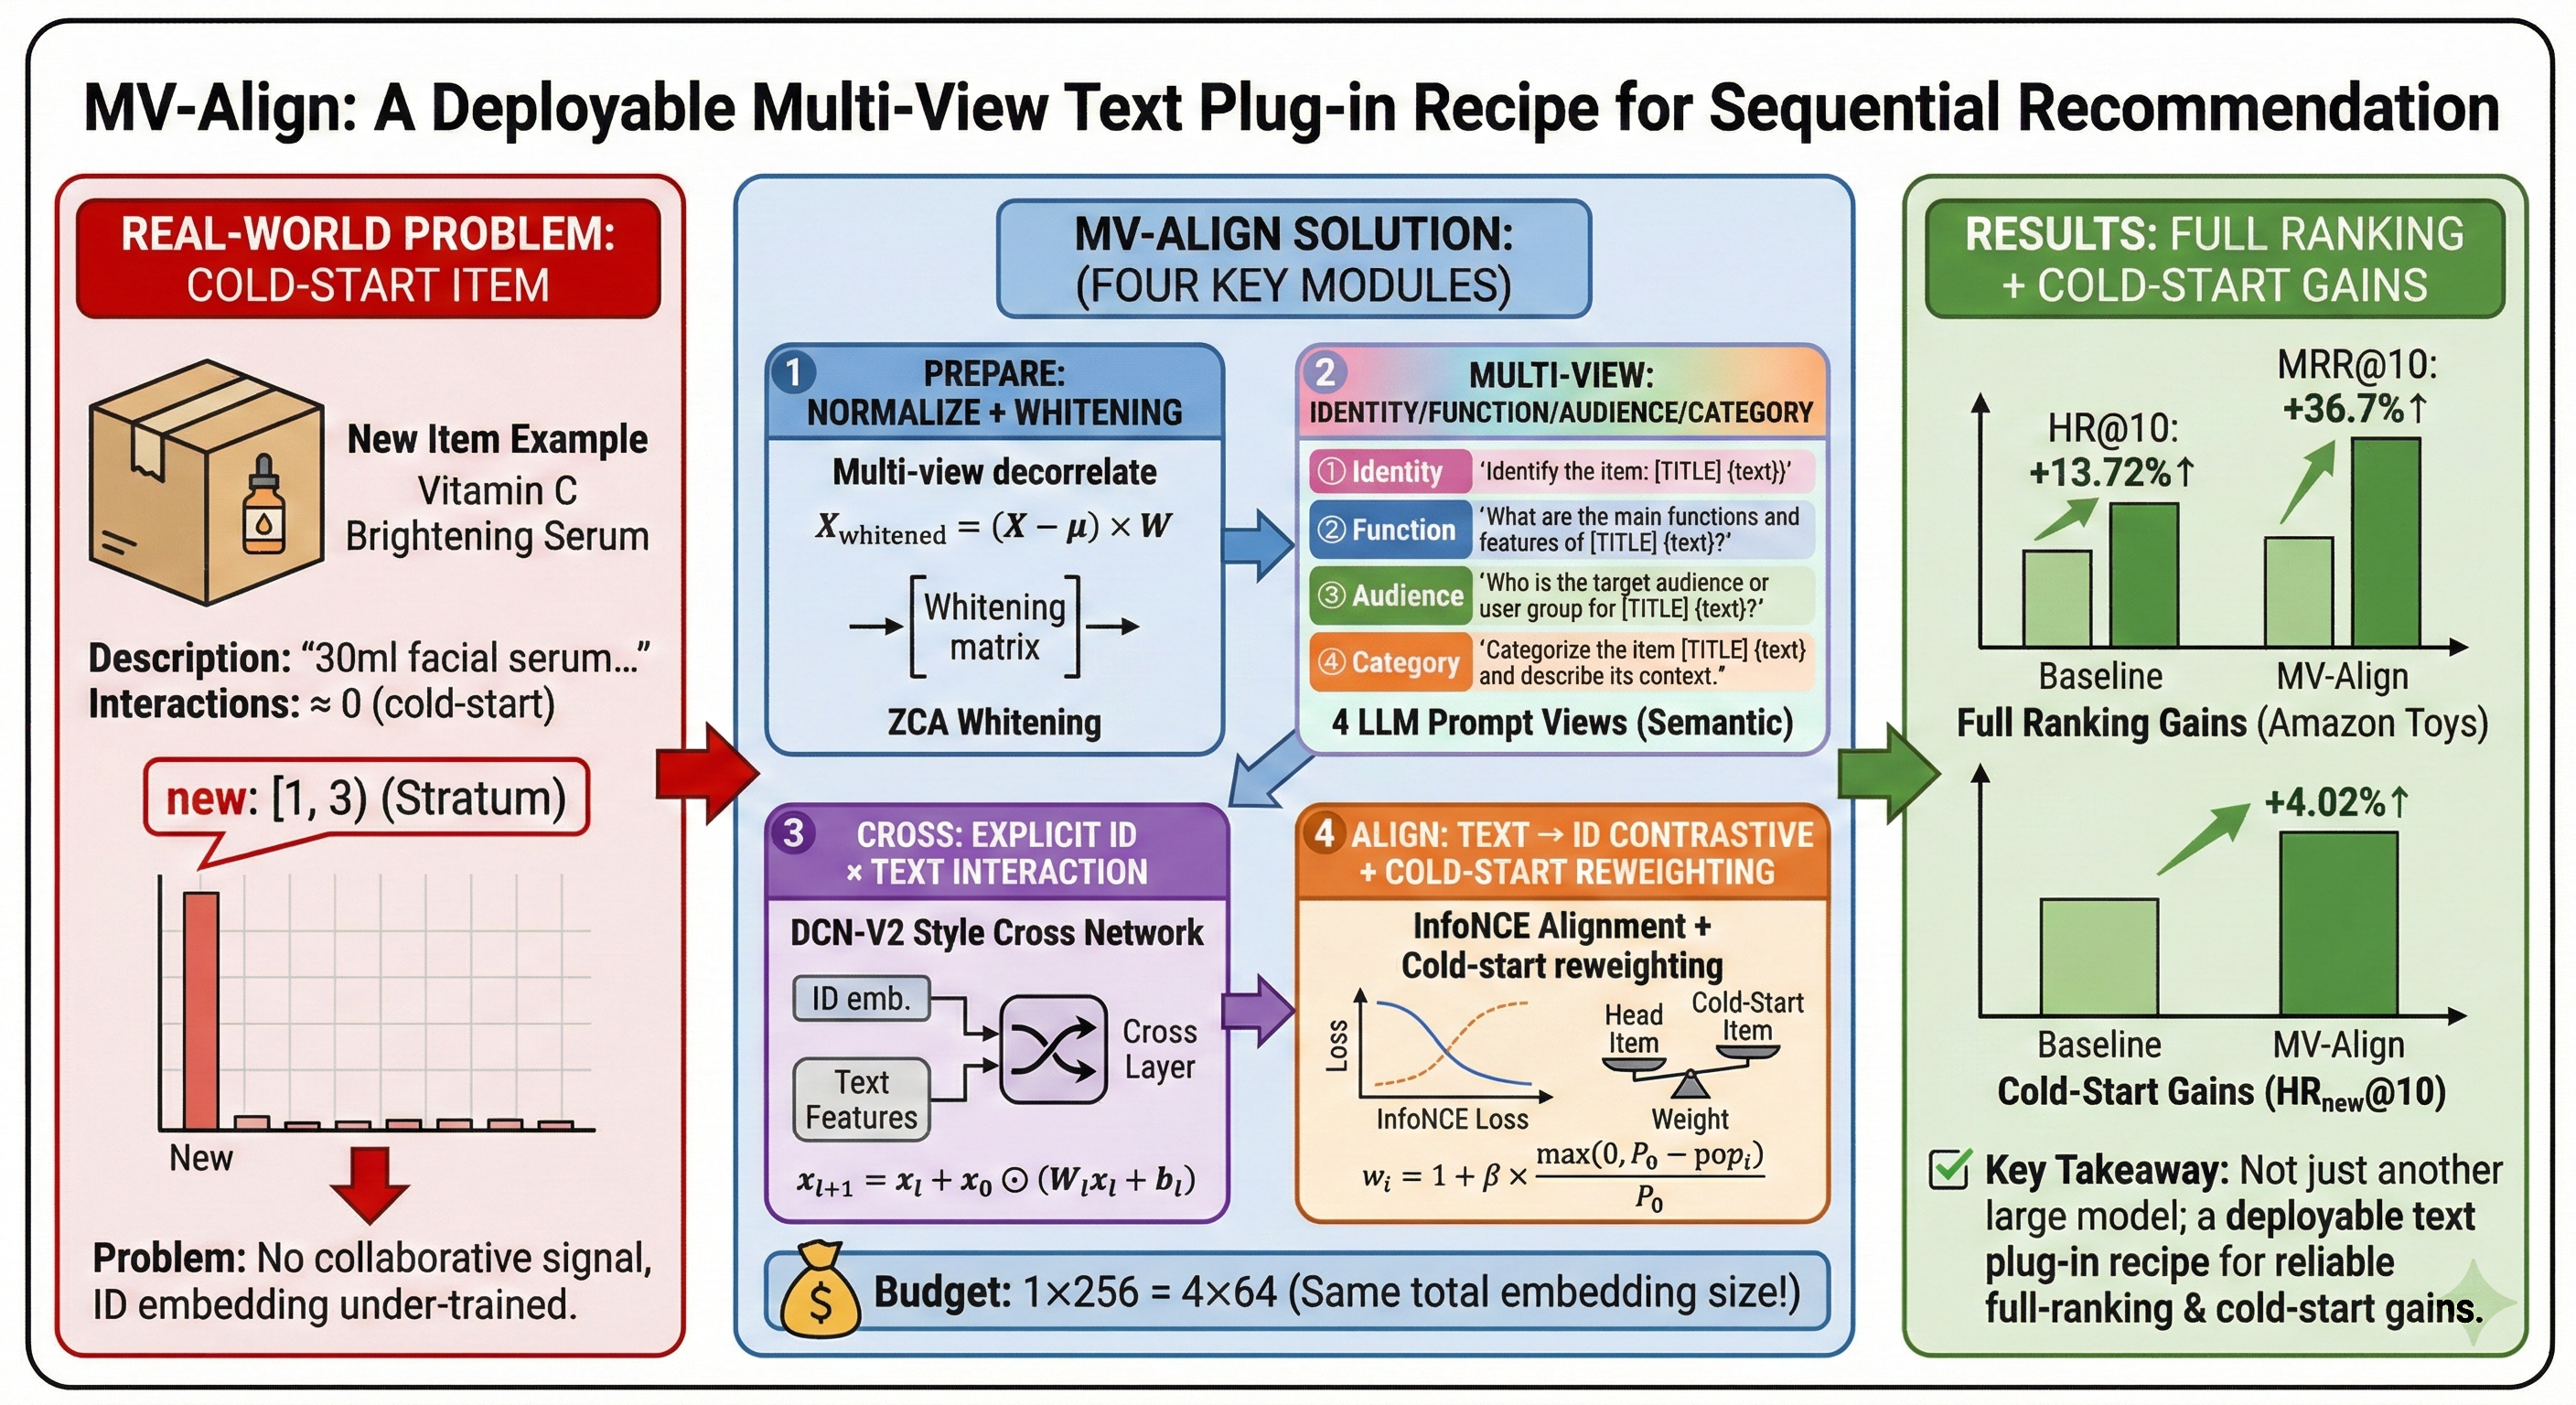
\includegraphics[width=0.95\textwidth]{figures/mv-cover.png}
\caption{Overview of \model: a deployable text plug-in for sequential recommendation.
\textbf{Left}: Cold-start items lack collaborative signals (new stratum: [1,3) interactions).
\textbf{Middle}: Four-module recipe---\textit{Prepare} (normalize+whiten), \textit{Multi-view} (4 LLM prompts), \textit{Cross} (DCN-V2 ID$\times$Text), and \textit{Align} (InfoNCE with cold-start reweighting).
\textbf{Right}: Full-ranking gains (+13.72\% HR@10, +36.7\% MRR@10) and cold-start improvements (+4.02\% HR\_new@10).
Budget: 1$\times$256-d = 4$\times$64-d (same total).}
\label{fig:cover}
\end{figure*}

%% TODO(sec_01): append the Research Questions from sec_03 as a closing
%%   paragraph or numbered list at the end of Introduction.

\section{Related Work}
\paragraph{Sequential recommendation.}
Transformer-based sequential models such as
\base~\cite{kang2018sasrec} and BERT4Rec~\cite{sun2019bert4rec}
(which adopts bidirectional masked prediction) are strong backbones for
capturing user behavior patterns.
GRU4Rec~\cite{hidasi2015gru4rec} pioneered RNN-based session
modeling, while SASRec introduced self-attention for next-item
prediction with causal masking. Recent efficient variants
include LightSANs~\cite{fan2021lightsans} with low-rank
attention decomposition for reduced complexity.

\paragraph{Text-enhanced recommendation.}
Item text features (from bag-of-words, neural encoders, or
\llm embeddings) provide complementary signals beyond
collaborative filtering. Early work used TF-IDF and
Item2Vec~\cite{barkan2016item2vec} for item representation;
CDL~\cite{wang2015cdl} jointly modeled text via stacked
denoising autoencoders. Recent approaches leverage pretrained
language models: UniSRec~\cite{hou2022unisrec} uses
BERT-encoded item text as universal transferable
representations, while VQ-Rec~\cite{hou2023vqrec} bridges
language and collaborative semantics via vector quantization.
Large language models have further expanded this line:
P5~\cite{geng2022p5} unifies recommendation in a text-to-text
paradigm, and TALLRec~\cite{bao2023tallrec} aligns LLMs with
recommendation via instruction tuning. However, these methods
typically encode item text with a single prompt or
representation; our work explores \emph{multi-view} \llm
embeddings via diverse prompt perspectives
(identity/function/audience/category) with explicit fusion and
alignment, and we show when this added complexity is justified
versus simpler alternatives.

\paragraph{Feature interaction and cross networks.}
Deep \& Cross Network (DCN)~\cite{wang2017dcn} and its
successor DCN-V2~\cite{wang2021dcnv2} explicitly model feature
crosses, complementing implicit interactions learned by DNNs.
Squeeze-and-Excitation Networks (SENet)~\cite{hu2018senet}
introduced channel-wise attention for adaptive feature
recalibration; FiBiNET~\cite{huang2019fibinet} adapted SENet
for CTR prediction with bilinear feature interactions. In
recommendation, cross networks have shown effectiveness in CTR
prediction; we adapt them for ID-text fusion in sequential
settings, and use SE-style blocks for per-view channel gating of \llm
features.

\paragraph{Multi-view learning in recommendation.}
Multi-view learning leverages complementary information from
different feature sources or modalities. Inspired by
CLIP~\cite{radford2021clip}, which aligns visual and textual
representations via contrastive learning, we design multi-view
prompts to elicit diverse semantics from language models. In
recommendation, multi-view approaches have been explored for
session-based settings~\cite{wang2023kgmvgnn} using
knowledge-enhanced graph neural networks. Our work applies
multi-view learning to \llm text embeddings, using different
prompt perspectives (identity, function, audience, category)
and whitening to decorrelate view representations before
fusion.

\paragraph{Contrastive learning in recommendation.}
Contrastive objectives such as \InfoNCE~\cite{oord2018cpc}
have been widely adopted for self-supervised representation
learning. In recommendation, contrastive methods align
user/item representations across views~\cite{wu2021cl4rec}.
We extend this to multi-view text-to-ID alignment with
cold-start reweighting.

\paragraph{Evaluation protocols.}
Sampled evaluation can mislead model
selection~\cite{krichene2020sampledmetrics}; full-ranking
evaluation provides more reliable comparisons but is
computationally expensive. We adopt full ranking with
stratified analysis to understand model behavior across
popularity strata.


%% sec_03 (Research Questions) — folded into Introduction.
%% \section{Research Questions}
We organize the study around the following research questions,
with a focus on \textbf{ablation studies} to understand when
and why each component helps:

\begin{itemize}[leftmargin=*,itemsep=3pt]
  \item \textbf{RQ1 (Whitening effect).}
    Does whitening (vs.\ L2-only normalization) improve
    text/\llm feature quality in single-view and multi-view
    settings?
  
  \item \textbf{RQ2 (SE-style channel attention).}
    Does SE-style channel gating provide effective channel attention for
    text features? We compare single-view and multi-view
    with/without SE-style blocks.
  
  \item \textbf{RQ3 (Multi-view vs.\ single-view).}
    Given the same total embedding dimension (e.g.,
    single-view 256-d vs.\ multi-view $4\times 64$-d), does
    multi-view prompting outperform single-view? We focus on
    HR@K, NDCG@K, MRR@K, especially on \textbf{new} and
    \textbf{few} item strata (cold-start items).
  
  \item \textbf{RQ4 (Cross and Align ablation).}
    What are the individual and combined contributions of
    explicit cross fusion and multi-view alignment? We ablate:
  \begin{itemize}[leftmargin=*,itemsep=1pt]
    \item multi-view + cross + align (full model)
    \item multi-view + cross (no align)
    \item multi-view + align (no cross)
    \item multi-view only (no cross, no align)
  \end{itemize}
\end{itemize}


\section{Method}
Figure~\ref{fig:framework} illustrates the overall architecture of \model.
The framework consists of three key components:
(1)~\textbf{Normalize \& Whiten}, where each text view undergoes per-view normalization to address anisotropy;
(2)~\textbf{Cross Network}, which captures explicit ID$\times$Text interactions via DCN-V2;
and (3)~\textbf{Multi-View Alignment}, which uses InfoNCE loss with cold-start reweighting to align text views with ID embeddings.
We elaborate each component below.

\subsection{Backbone: SASRec with Text Fusion}
Let a user interaction sequence be $s_u = [i_1,\dots,i_n]$
with maximum length $L$. \base encodes $s_u$ into a sequence
representation $\mathbf{h}_u \in \mathbb{R}^d$ via a
Transformer. Each item $i$ has an ID embedding
$\mathbf{e}_i \in \mathbb{R}^d$. We augment items with text
features and fuse them into a \emph{fused item embedding}
$\tilde{\mathbf{e}}_i$ used for scoring.

\subsection{Multi-View Text Representations}
We assume a lightweight \tfidf embedding $\mathbf{t}_i^{(0)} \in \mathbb{R}^{d_t}$
as a base view and $V$ \llm prompt views
$\{\mathbf{t}_i^{(v)} \in \mathbb{R}^{d_l}\}_{v=1}^V$ (e.g.,
identity/function/audience/category views), where $d_t$ and $d_l$ denote the
\tfidf and raw \llm embedding dimensions, respectively.

\paragraph{Per-view whitening.}
Multi-view \llm embeddings suffer from three failure modes:
\textbf{(i) scale mismatch}---different views may have vastly
different magnitude distributions, causing some views to
dominate fusion; \textbf{(ii) view correlation}---prompts
eliciting similar semantics produce correlated features that
redundantly encode the same information; \textbf{(iii)
cross-view redundancy}---without decorrelation, the cross
network learns redundant interactions across views rather than
complementary feature crosses.

To address these issues, we first reduce each \llm view from $d_l$ to $d_v$
dimensions via truncated SVD, then apply ZCA whitening~\cite{kessy2018zca} to each view
independently, which decorrelates multi-view channels and makes
subsequent interactions more learnable.
Given the reduced embedding matrix $\mathbf{X}^{(v)} \in \mathbb{R}^{|I| \times d_v}$
for view $v$ over all items, we compute:
\begin{align}
  \mathbf{X}_c^{(v)} &= \mathbf{X}^{(v)} - \boldsymbol{\mu}^{(v)}, \\
  \boldsymbol{\Sigma}^{(v)} &= \frac{1}{|I|}(\mathbf{X}_c^{(v)})^\top \mathbf{X}_c^{(v)}, \\
  \mathbf{X}_w^{(v)} &= \mathbf{X}_c^{(v)} (\boldsymbol{\Sigma}^{(v)} + \epsilon \mathbf{I})^{-1/2},
\end{align}
where $\boldsymbol{\mu}^{(v)}$ is the mean embedding, $\boldsymbol{\Sigma}^{(v)}$
is the covariance matrix, and $\epsilon$ is a small constant for numerical
stability. The whitening statistics are computed offline on the training set
and fixed during training/inference. Each view uses its own whitening
parameters (per-view whitening), which better preserves view-specific
semantics than shared whitening across views.

\paragraph{SE-style channel gating.}
We use an SE-style channel gating for adaptive feature
recalibration, inspired by the channel-wise attention mechanism
in SENet~\cite{hu2018senet}. While the original SENet applies
squeeze (global pooling) followed by excitation, our
implementation directly applies an MLP-based gating over each
projected embedding, which is more suitable for per-item
representations (no pooling across items). Each whitened view
is projected to the backbone dimension $d$ and refined by:
\begin{align}
  \mathbf{z}_i^{(v)} &= \mathbf{W}_v \mathbf{t}_{w,i}^{(v)} \in \mathbb{R}^d,\\
  \mathbf{r}_i^{(v)} &= \mathbf{z}_i^{(v)} \odot \sigma(\mathrm{MLP}_v(\mathbf{z}_i^{(v)})),
\end{align}
where $\mathbf{W}_v \in \mathbb{R}^{d \times d_v}$ is the projection matrix,
$\mathbf{t}_{w,i}^{(v)} \in \mathbb{R}^{d_v}$ is the whitened embedding for
item $i$ in view $v$, and $\mathrm{MLP}_v: \mathbb{R}^d \to \mathbb{R}^d$ is a two-layer
network with reduction ratio $r$.

\paragraph{Per-view $\ell_2$ normalization.}
After SE-style gating, we apply per-view $\ell_2$ normalization
to each view independently. This normalization serves two purposes:
(i) it ensures each view contributes to the fusion on a comparable
scale, preventing views with larger magnitudes from dominating;
(ii) it stabilizes the subsequent cross network learning by
providing well-conditioned inputs:
\begin{equation}
  \hat{\mathbf{r}}_i^{(v)} = \frac{\mathbf{r}_i^{(v)}}{\lVert \mathbf{r}_i^{(v)} \rVert_2 + \epsilon}.
\end{equation}
Together with whitening, per-view normalization addresses scale mismatch
across views while preserving their distinct semantic content: whitening
decorrelates feature dimensions within each view, while $\ell_2$
normalization ensures comparable contribution magnitudes across views.

\paragraph{View gating and fusion.}
We learn a scalar gate $g_v=\sigma(\theta_v)\in(0,1)$ for each
view and \emph{do not} enforce cross-view normalization (each
view independently contributes $0$--$1$). All views (and
optionally the \tfidf base) are concatenated and projected
back to $\mathbb{R}^d$:
\begin{equation}
  \mathbf{t}_i = \mathbf{P}\Big[\mathbf{t}_i^{(0)};\; g_1\hat{\mathbf{r}}_i^{(1)};\; \dots;\; g_V\hat{\mathbf{r}}_i^{(V)}\Big] \in \mathbb{R}^d,
\end{equation}
where $\mathbf{P} \in \mathbb{R}^{d \times (d_t + Vd)}$ is the fusion projection matrix.

\subsection{Explicit Cross Fusion}
Rather than relying solely on self-attention to capture
high-order interactions between collaborative and textual
signals, we introduce an \emph{explicit cross} module based on
DCN-V2~\cite{wang2021dcnv2}. Self-attention in \base models
sequence-level item--item dependencies, but does not
explicitly model feature-level crosses between ID embeddings
and text embeddings. DCN-V2 cross networks fill this gap by
learning high-order ID$\times$text interactions through
element-wise products gated by learned weight matrices.

Given concatenated features
$\mathbf{x}_i=[\mathbf{e}_i;\alpha_i \mathbf{t}_i] \in \mathbb{R}^{2d}$, where
$\mathbf{e}_i \in \mathbb{R}^d$ is the ID embedding and $\mathbf{t}_i \in \mathbb{R}^d$ is the
fused text representation, a cross layer updates:
\begin{equation}
  \mathbf{x}^{(l+1)} = \mathbf{x}^{(l)} + \mathbf{x}^{(0)} \odot (\mathbf{W}_l\mathbf{x}^{(l)} + \mathbf{b}_l),
\end{equation}
where $\mathbf{W}_l \in \mathbb{R}^{2d \times 2d}$ is a
full-rank weight matrix and $\mathbf{b}_l \in \mathbb{R}^{2d}$ is the bias;
$\odot$ denotes element-wise product. We use the full-rank variant of DCN-V2 (non-mix)
rather than low-rank or mixture-of-experts variants. The
cross output $\mathbf{x}^{(C)} \in \mathbb{R}^{2d}$ is combined with a shallow MLP via a predictor
layer to produce the fused embedding $\tilde{\mathbf{e}}_i \in \mathbb{R}^d$.
The scalar $\alpha_i \in (0,1)$ includes a global text gate and
optional per-item gating, scaled by temperature for stable
fusion.

\subsection{Multi-View Contrastive Alignment}
We align each text view to the ID embedding space using
\InfoNCE~\cite{oord2018cpc}. The alignment objective is:
\textbf{text view $\to$ ID space}; positive pairs are
(item's text view, item's ID embedding); negatives are
in-batch items. This ensures that text representations
carry collaborative signals and can serve as drop-in
replacements for ID embeddings in cold-start scenarios.

For a batch of $B$ items, we define
the cosine similarity matrix
$\mathbf{S} \in \mathbb{R}^{B \times B}$ with entries
$\mathbf{S}_{ij} = \mathrm{cos}(\mathbf{e}_{i},
\hat{\mathbf{r}}_{j}^{(v)})$ between ID embeddings
$\mathbf{e}_i \in \mathbb{R}^d$ and text view embeddings
$\hat{\mathbf{r}}_j^{(v)} \in \mathbb{R}^d$, with temperature $\tau$.
The per-view alignment loss is:
\begin{equation}
  \mathcal{L}_{\text{align}}^{(v)} =
  \frac{1}{B}\sum_{i=1}^{B}
  -\log \frac{\exp(\mathbf{S}_{ii}/\tau)}{\sum_{j=1}^{B}\exp(\mathbf{S}_{ij}/\tau)}.
\end{equation}
We learn view weights $\pi_v=\mathrm{softmax}(\boldsymbol{\phi})_v$
and combine per-view losses:
\begin{equation}
  \mathcal{L}_{\text{mv-align}} = \sum_{v=1}^{V}\pi_v \mathcal{L}_{\text{align,w}}^{(v)}.
\end{equation}

We enhance cold-start item performance through two complementary
mechanisms that operate at different stages:

\paragraph{Training-time cold-start reweighting.}
To avoid alignment being dominated by frequent items, we
reweight samples based on item popularity $\mathrm{pop}(i)$
during training, where $\mathrm{pop}(i)$ is the interaction count:
\begin{equation}
  w_i = 1 + \beta\cdot \max\Big(0, \frac{P_0-\mathrm{pop}(i)}{P_0}\Big),
\end{equation}
where $P_0$ is the cold-start threshold (items with $\mathrm{pop}(i) < P_0$
receive boosted weights). The weighted alignment loss becomes:
\begin{equation}
  \mathcal{L}_{\text{align,w}}^{(v)} =
  \frac{1}{\sum_i w_i}\sum_{i=1}^{B} w_i \cdot
  \left[-\log \frac{\exp(\mathbf{S}_{ii}/\tau)}{\sum_{j=1}^{B}\exp(\mathbf{S}_{ij}/\tau)}\right],
\end{equation}
where $w_i$ only reweights the anchor (positive) samples, ensuring
that cold-start items receive sufficient gradient updates during
alignment training.

\paragraph{Inference-time cold-start boosting.}
To complement training-time reweighting, we apply adaptive text
weighting during inference. For an item $i$ with popularity
$\mathrm{pop}(i)$, we compute a dynamic boost factor:
\begin{equation}
  \gamma_i = 1 + \beta_{\text{infer}} \cdot \max\Big(0, 
  \frac{P_0-\mathrm{pop}(i)}{P_0}\Big),
  \label{eq:infer_boost}
\end{equation}
where $\beta_{\text{infer}}$ is the inference boost coefficient.
The effective text weight in the fusion layer becomes 
$\alpha_i' = \alpha_i \cdot \gamma_i$, dynamically increasing text
reliance for cold-start items without modifying model parameters.
This decoupling allows deployment-time adjustment without
retraining: lower $\beta_{\text{infer}}$ for balanced performance,
or higher $\beta_{\text{infer}}$ for cold-start prioritization
(see Appendix~\ref{app:hyper} for validated configurations).

Together, these two mechanisms ensure that cold-start items receive
both strong learning signals during training (via reweighted
alignment) and appropriate inference-time emphasis (via dynamic
boosting), enabling effective cold-start recommendations without
sacrificing performance on frequent items.

\begin{figure}[t]
\centering
\IfFileExists{figures/framework.pdf}{%
  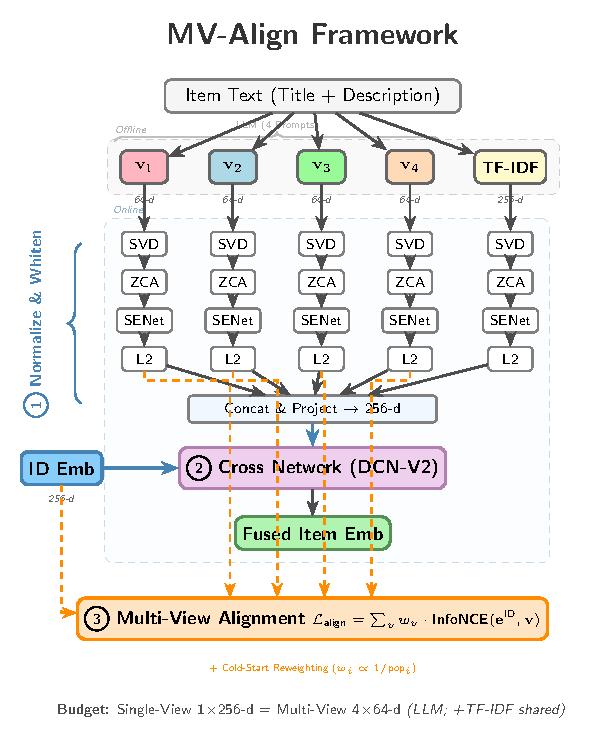
\includegraphics[width=\linewidth]{figures/framework.pdf}%
}{%
  \fbox{\parbox[c][0.22\textheight][c]{0.95\linewidth}{\centering
  \textbf{Framework figure placeholder.}\\
  Put `framework.pdf` under `paper_sigir/figures/`.}}%
}
\caption{Overview of the MV-Align framework. The architecture consists of three key components:
\circled{1}~\textbf{Normalize \& Whiten}: each view (4 LLM prompts + TF-IDF) undergoes SVD, ZCA whitening, SE-style gating, and L2 normalization;
\circled{2}~\textbf{Cross Network}: DCN-V2 captures explicit ID$\times$Text interactions;
\circled{3}~\textbf{Multi-View Alignment}: InfoNCE loss with cold-start reweighting aligns each view to ID embeddings.
Embedding budget: single-view uses 1$\times$256-d while multi-view uses 4$\times$64-d (LLM only; TF-IDF 256-d shared).}
\label{fig:framework}
\end{figure}

\subsection{Training Objective}
We optimize:
\begin{equation}
  \mathcal{L} = \mathcal{L}_{\text{rec}} + \lambda \cdot \mathcal{L}_{\text{mv-align}},
\end{equation}
where $\mathcal{L}_{\text{rec}}$ is the standard sequential
recommendation loss (cross-entropy over sampled
positives/negatives in training), and $\lambda$ is the
alignment weight.

\subsection{Model Complexity}
We analyze the space (parameter) and time complexity of each
model variant, following the analysis in~\cite{kang2018sasrec}.
Let $|I|$ denote the number of items, $L$ the maximum sequence
length, $d$ the hidden size, $B$ the batch size, $d_t$ the
\tfidf feature dimension, $d_l$ the \llm embedding dimension,
$V$ the number of text views, and $d_v$ the per-view \llm
dimension.

\paragraph{Space complexity (parameters).}
Table~\ref{tab:complexity} summarizes the parameter and time complexity for each configuration:

\begin{table*}[t]
\caption{Parameter and time complexity of model variants.
$|I|$: \#items, $L$: sequence length, $d$: hidden size,
$d_t$: \tfidf dim, $d_l$: \llm dim, $V$: \#views, $d_v$: per-view dim.}
\label{tab:complexity}
\centering
\small
\begin{tabular}{lll}
\toprule
\textbf{Model} & \textbf{Space Complexity (Parameters)} & \textbf{Time Complexity (per batch)} \\
\midrule
\base (ID-only) & $O(|I|d + Ld + d^2)$ & $O(L^2d + Ld^2 + |I|d)$ \\
\base + \tfidf & $O(|I|d + Ld + d^2 + d_t d)$ & $O(L^2d + Ld^2 + |I|d_t d + |I|d)$ \\
\base + \tfidf + \llm (single-view) & $O(|I|d + Ld + d^2 + (d_t{+}d_l)d)$ & $O(L^2d + Ld^2 + |I|(d_t{+}d_l)d + |I|d)$ \\
\model (multi-view) & $O(|I|d + Ld + d^2 + Vd_v d + d_t d)$ & $O(L^2d + Ld^2 + V|I|d_v d + |I|d)$ \\
\bottomrule
\end{tabular}
\end{table*}

\paragraph{Space breakdown.}
The \base backbone contributes $O(|I|d)$ for item embeddings,
$O(Ld)$ for position embeddings, and $O(d^2)$ for the
Transformer encoder parameters (self-attention $Q,K,V,O$
projections and point-wise FFN layers; the number of layers
is a small constant). Text variants add projection layers
proportional to the text feature dimension: \tfidf adds
$O(d_t d)$, single-view \llm adds $O((d_t + d_l)d)$, and
multi-view adds $O(V d_v d)$ for per-view projections and
SE-style gating modules plus $O(d_t d)$ for the base view. Cross layers
contribute $O(d^2)$ each (we use a single cross layer),
absorbed into the backbone $O(d^2)$ term.

\paragraph{Time breakdown.}
The Transformer self-attention layer costs $O(L^2d)$ for
computing the $L\times L$ attention matrix, plus $O(Ld^2)$
for the point-wise FFN. Full-ranking scoring adds $O(|I|d)$
for computing logits over all items. Text models incur
additional fusion overhead:
\begin{itemize}[leftmargin=*,itemsep=1pt]
  \item \textbf{\tfidf}: Text projection $O(|I| d_t d)$ for all items.
    Cross network fusion is $O(|I| d^2)$, absorbed since $d_t \approx d$.
  \item \textbf{Single-view}: Projection cost increases to
    $O(|I| (d_t + d_l) d)$ due to larger input dimension.
  \item \textbf{Multi-view}: Per-view projection $O(V |I| d_v d)$;
    concat and cross costs are absorbed since $V d_v \approx d_t \approx d$.
\end{itemize}
Alignment loss adds $O(B^2 d)$ per view for InfoNCE similarity
matrix computation. Note that \llm embeddings are
\emph{precomputed offline} and stored as static buffers; the
online inference cost is dominated by projection layers
rather than the \llm encoder.

%% TODO(sec_04): absorb sec_05 (Two-Phase Training Protocol) as a short
%%   subsection at the end of Method; keep it concise (offline vs online,
%%   2-3 sentences + Algorithm box only if space permits).

%% sec_05 (Two-Phase Training Protocol) — folded into Method.
%% \section{Two-Phase Training Protocol}
We use a two-phase training protocol that jointly learns text
representations and the backbone from the start:
\begin{itemize}[leftmargin=*,itemsep=2pt]
  \item \textbf{Phase-A (text warmup).}
    Initialize both backbone and text modules together;
    freeze the backbone and train text heads and cross modules
    with a higher learning rate;
    grid-search $(\lambda,\tau)$ by a validation metric.
  \item \textbf{Phase-B (joint finetune).}
    Unfreeze the backbone and finetune all parameters
    with grouped learning rates (text head, cross/DNN, backbone).
\end{itemize}
\paragraph{Joint initialization rationale.}
We initialize text and backbone modules together rather than
pre-training the ID backbone alone. Starting with both modalities
from epoch 0 ensures that text heads receive sufficient learning
signals while ID embeddings remain adaptable to text-augmented
representations, facilitating effective multi-modal fusion.


\section{Experiments}
\subsection{Datasets and Evaluation}
We evaluate on two Amazon product review domains~\cite{mcauley2015amazon,ni2019amazon}: \textbf{Beauty} and
\textbf{Toys\&Games}. We follow time-ordered splits and
report metrics under \textbf{full ranking} at $K\in\{5,10,20\}$.
In addition to overall metrics (HR, NDCG, MRR, Precision),
we report \textbf{popularity-stratified} metrics by item
interaction counts:
\begin{itemize}[leftmargin=*,itemsep=1pt]
  \item \textbf{new}: $[1,3)$ interactions
  \item \textbf{few}: $[3,10)$ interactions
  \item \textbf{frequent}: $[10,\infty)$ interactions
\end{itemize}
We compute popularity strata from item interaction counts in
the training data. We focus on full-ranking metrics in the
main paper and omit uni100-style sampled metrics for clarity
and reliability; Appendix~\ref{app:sampled} provides a sanity
check comparing sampled vs.\ full ranking. Our evaluation
follows leave-one-out next-item prediction with a single
ground-truth item per test case, under which HR@K, Hit@K, and
Recall@K coincide; we use HR@K for brevity and rely on
MRR/NDCG to capture top-position quality.

\subsection{Baselines}
We compare four primary configurations:
\begin{itemize}[leftmargin=*,itemsep=2pt]
  \item \textbf{\base (ID-only).} Pure sequential baseline
    without text/cross/align.
  \item \textbf{\base + \tfidf.} A lightweight text baseline
    using precomputed \tfidf embeddings with explicit cross
    and alignment.
  \item \textbf{\base + \tfidf + \llm (single-view).} Adds a
    single \llm embedding (Qwen2.5-7B~\cite{qwen2024qwen25}) concatenated with
    \tfidf, using SE-style gating and alignment.
  \item \textbf{\model (multi-view).} \tfidf base view + 4
    multi-view \llm prompt embeddings
    (identity/function/audience/category) with per-view SE-style blocks,
    explicit cross, and multi-view contrastive alignment.
\end{itemize}
We further include representative sequential baselines (e.g.,
BERT4Rec~\cite{sun2019bert4rec}, S3-Rec~\cite{zhou2020s3rec},
FDSA~\cite{zhang2019fdsa}, UniSRec~\cite{hou2022unisrec},
GRU4Rec~\cite{hidasi2016gru4rec})
and lightweight text encoders as additional comparisons.
When reporting a third domain, we additionally use
Book-Crossing~\cite{ziegler2005bookcrossing}.

\subsection{Implementation Details}
Unless stated otherwise, we use embedding size $d=256$, max
sequence length $L=50$, 2 Transformer layers with 2 heads,
batch size 512, and Adam with base learning rate $10^{-4}$.
\paragraph{Two-phase schedule.}
We follow Phase-A ($15$ epochs) $\rightarrow$ Phase-B ($50$
epochs) with Phase-A selecting $(\lambda,\tau)$ on
\texttt{MRR@10} for Beauty and \texttt{HR@10} for Toys\&Games.
We use grouped learning rates:
$\text{lr}_{\text{text}}=\num{1e-3}$ for text heads,
$\text{lr}_{\text{cross}}=\num{5e-4}$ for cross/DNN blocks,
and $\text{lr}_{\text{backbone}}=\text{lr}_{\text{text}}\times
0.1$ in Phase-B.
\paragraph{Grid.}
For the main runs, we use the Aggressive configuration:
$\lambda=0.10$ and $\tau=0.05$ on both datasets
(see Table~\ref{tab:hyper_config} for complete hyperparameter
settings including cold-start boosting); additional grids can
be enabled via the training script.
\paragraph{Reproducibility.}
We use seed 2025 and report full-ranking metrics over
$K\in\{5,10,20\}$ with popularity stratification thresholds
\texttt{new}:[1,3), \texttt{few}:[3,10),
\texttt{frequent}:[10,$\infty$). Our implementation is based on
RecBole~\cite{zhao2021recbole}; all exact settings are
reproducible from the provided YAML configs and run scripts
in the repository.

\paragraph{Parameter counts.}
Table~\ref{tab:params} shows the actual trainable parameter
counts on Amazon Beauty ($|I|=12,102$, $d=256$, $d_t=256$,
$d_l=1024$, $V=4$, $d_v=1024$).
The multi-view model adds only modest overhead (${\sim}6$M
params) over the single-view baseline, while the \llm
embeddings themselves are precomputed offline and stored as
static buffers (not counted as trainable parameters).

\begin{table}[h]
\caption{Trainable parameter counts (Amazon Beauty).}
\label{tab:params}
\centering
\small
\begin{tabular}{lrr}
\toprule
\textbf{Model} & \textbf{\#Params} & \textbf{Overhead} \\
\midrule
\base (ID-only) & ${\sim}3.5$M & --- \\
\base + \tfidf & ${\sim}4.5$M & +1.0M \\
\base + \tfidf + \llm & ${\sim}5.3$M & +1.8M \\
\model (multi-view) & ${\sim}11.5$M & +8.0M \\
\bottomrule
\end{tabular}
\end{table}


\section{Main Results}
Table~\ref{tab:main} reports full-ranking results on Beauty
and Toys\&Games. Across both datasets, adding text features
consistently improves over the ID-only baseline, with \tfidf
providing substantial gains (+2.6\% HR@10 on Beauty, +6.2\%
on Toys). The key findings are:

\paragraph{Text features provide large gains over ID-only.}
On Beauty, \tfidf alone improves HR@10 from 5.42\% to 5.56\%
(+2.6\%), and NDCG@10 from 2.93\% to 3.69\% (+26.0\%). On
Toys, \tfidf improves HR@10 from 5.92\% to 6.29\% (+6.2\%)
and NDCG@10 from 3.30\% to 4.26\% (+29.1\%).


\paragraph{Multi-view shows consistent improvements.}
\model (7B) achieves the best performance on both datasets.
On \textbf{Beauty}, \model achieves HR@10=5.79\% (+6.8\% vs
ID-only), with MRR@10=3.19\% and NDCG@10=3.80\%. On
\textbf{Toys}, \model achieves HR@10=6.61\% (+11.7\% vs
ID-only), NDCG@10=4.39\%, MRR@10=3.71\%. The hierarchy
\model $>$ TF-IDF+LLM $>$ TF-IDF $>$ ID-only holds for all
overall metrics on both datasets.

\paragraph{Cold-start (new/few) improvements.}
For the \textbf{new} stratum, \model achieves HR\_new@10=1.76\%
(Beauty) and 2.04\% (Toys), recovering or exceeding ID-only
(1.88\% and 1.92\%) while TF-IDF variants achieve slightly
lower HR\_new@10 (1.63\% and 1.83\%) due to aggressive
cold-start boosting that sharpens score distributions for
ranking quality at the cost of recall coverage.


\begin{table*}[t]
\caption{Main results under full ranking (mean$\pm$std over 4 seeds). Best results per dataset in \textbf{bold}; $^{**}$/$^{*}$ denotes paired $t$-test significance at $p<0.01$/$p<0.05$ vs.\ the strongest baseline (TF-IDF+LLM). All values are percentages (\%). Extended strata results in Appendix~\ref{app:strata}.}
\label{tab:main}
\centering
\small
\begin{tabular}{lcccccc}
\toprule
\multirow{2}{*}{\textbf{Model}} &
\multicolumn{3}{c}{\textbf{Overall}} &
\multicolumn{3}{c}{\textbf{new stratum} $[1,3)$} \\
\cmidrule(lr){2-4}\cmidrule(lr){5-7}
& HR@10 & NDCG@10 & MRR@10 & HR@10 & NDCG@10 & MRR@10 \\
\midrule
\multicolumn{7}{l}{\textbf{Amazon Beauty}} \\
\base (ID-only, 50ep) & 5.42$\pm$0.21 & 2.93$\pm$0.05 & 2.14$\pm$0.01 & 1.88$\pm$0.03 & 1.05$\pm$0.02 & 0.78$\pm$0.02 \\
\base + \tfidf & 5.56$\pm$0.03 & 3.69$\pm$0.02 & 3.11$\pm$0.01 & 1.63$\pm$0.02 & 1.21$\pm$0.03 & 1.08$\pm$0.03 \\
\base + \tfidf + \llm (7B) & 5.62$\pm$0.03 & 3.73$\pm$0.02 & 3.15$\pm$0.01 & 1.64$\pm$0.03 & 1.24$\pm$0.02 & 1.11$\pm$0.02 \\
\model (7B) & \textbf{5.79}$^{**}$$\pm$0.04 & \textbf{3.80}$^{**}$$\pm$0.02 & \textbf{3.19}$^{*}$$\pm$0.02 & \textbf{1.76}$\pm$0.05 & \textbf{1.28}$\pm$0.02 & \textbf{1.12}$\pm$0.03 \\
\midrule
\multicolumn{7}{l}{\textbf{Amazon Toys\&Games}} \\
\base (ID-only, 50ep) & 5.92$\pm$0.03 & 3.30$\pm$0.02 & 2.48$\pm$0.02 & 1.92$\pm$0.03 & 1.08$\pm$0.02 & 0.81$\pm$0.02 \\
\base + \tfidf & 6.29$\pm$0.03 & 4.26$\pm$0.01 & 3.64$\pm$0.01 & 1.83$\pm$0.03 & 1.38$\pm$0.02 & 1.23$\pm$0.02 \\
\base + \tfidf + \llm (7B) & 6.39$\pm$0.02 & 4.32$\pm$0.01 & 3.67$\pm$0.01 & 1.89$\pm$0.05 & 1.41$\pm$0.03 & 1.26$\pm$0.02 \\
\model (7B) & \textbf{6.61}$^{**}$$\pm$0.03 & \textbf{4.39}$^{*}$$\pm$0.03 & \textbf{3.71}$\pm$0.02 & \textbf{2.04}$\pm$0.03 & \textbf{1.47}$\pm$0.02 & \textbf{1.29}$\pm$0.02 \\
\bottomrule
\end{tabular}
\end{table*}

\subsection{Prompt Templates for Text Embeddings}
We describe the prompt templates used to generate text
embeddings from the LLM encoder (Qwen2.5).

\paragraph{Single-view embedding.}
For single-view LLM embeddings, we use a simple title-based
prompt:
\begin{quote}
\texttt{[TITLE] \{text\}}
\end{quote}
where \texttt{\{text\}} is the item title. The LLM encoder
processes this prompt and we extract the mean-pooled hidden
states as the item embedding.

\paragraph{Multi-view embeddings.}
For multi-view embeddings, we design four prompts capturing
different semantic perspectives:
\begin{enumerate}[leftmargin=*,itemsep=1pt]
  \item \textbf{Identity/Title}:
    \texttt{Identify the item: [TITLE] \{text\}}
  \item \textbf{Function/Utility}:
    \texttt{What are the main functions and features of
    [TITLE] \{text\}?}
  \item \textbf{Target Audience}:
    \texttt{Who is the target audience or user group for
    [TITLE] \{text\}?}
  \item \textbf{Category/Context}:
    \texttt{Categorize the item [TITLE] \{text\} and describe
    its context.}
\end{enumerate}
Each view is independently encoded, projected via SVD to 64
dimensions, and then processed through per-view SE-style gating
before fusion.
This design encourages the model to capture complementary
semantic aspects (what the item is, what it does, who uses
it, and how it fits into the catalog).

%% TODO(sec_07+08): merge into one "Results and Analysis" section.
%%   Main text keeps: main table (placeholder), trade-off figure, key ablation.

\section{Analysis}

We conduct systematic ablation studies to answer RQ1--RQ4.
All ablations use multi-view 7B with Aggressive configuration
on Toys, with relative changes derived from ablation
experiments.

\subsection{RQ1, RQ2 \& RQ4: Component Ablation}

Table~\ref{tab:ablation} presents ablation results for SE-style gating,
cross network, and whitening on Toys\&Games (7B, Aggressive configuration).

\begin{table}[t]
\caption{Component ablation on Toys\&Games (7B). All values in \%.}
\label{tab:ablation}
\centering
\scriptsize
\begin{tabular}{@{}lcccc@{}}
\toprule
\textbf{Configuration} & HR@10 & NDCG@10 & MRR@10 & HR\_new@10 \\
\midrule
\multicolumn{5}{l}{\textit{SE-style \& Cross Network (RQ2 \& RQ4)}} \\
Full (SE + Cross) & 6.92 & 4.51 & 3.76 & 1.99 \\
$-$ SE-style & 6.99 (+1.0\%) & 4.51 (0\%) & 3.72 ($-$1.0\%) & 2.06 (+3.3\%) \\
$-$ Cross & 7.50 (+8.4\%) & 4.30 ($-$4.7\%) & 3.28 ($-$12.7\%) & 2.28 (+14.8\%) \\
$-$ SE $-$ Cross & 7.52 (+8.6\%) & 4.28 ($-$5.0\%) & 3.27 ($-$13.1\%) & 2.30 (+15.8\%) \\
\midrule
\multicolumn{5}{l}{\textit{Whitening Effect (RQ1)}} \\
Multi-view w/ Whiten & 6.92 & 4.51 & 3.76 & 1.99 \\
Multi-view w/o Whiten & 6.76 ($-$2.3\%) & 4.48 ($-$0.7\%) & 3.77 (+0.3\%) & 1.96 ($-$1.5\%) \\
Single-view w/ Whiten & 6.61 & 4.42 & 3.74 & 1.96 \\
Single-view w/o Whiten & 6.59 ($-$0.3\%) & 4.41 ($-$0.2\%) & 3.74 (0\%) & 1.93 ($-$1.5\%) \\
\bottomrule
\end{tabular}
\end{table}

\paragraph{Cross Network is essential for ranking quality (RQ4).}
Removing the cross module increases HR@10 (+8.4\%) but \emph{sharply degrades}
ranking metrics: MRR@10 drops by 12.7\%, NDCG@10 drops by 4.7\%.
This reveals a fundamental \textbf{HR--ranking trade-off}: without
explicit cross interactions, the model produces smoother score
distributions that improve coverage but lose discriminative power
for top-1 ranking. Removing cross also improves HR\_new@10 (+14.8\%),
confirming that the cross module emphasizes frequent items.

\paragraph{SE-style gating has minor impact (RQ2).}
Removing SE-style gating alone causes only marginal changes ($<$3\% on
most metrics). The combination of removing both SE and Cross
shows the largest HR\_new@10 gains (+15.8\%), indicating that these
components together calibrate toward frequent items.

\paragraph{Whitening benefits multi-view but not single-view (RQ1).}
For multi-view, removing whitening reduces HR@10 by 2.3\% (6.92\% $\to$ 6.76\%),
while MRR@10 slightly improves (+0.3\%). This reveals that whitening primarily
benefits recall coverage by decorrelating multi-view features.
For single-view (TF-IDF+LLM), removing whitening has minimal impact
(HR@10 $-$0.3\%, MRR 0\%), confirming that single-view LLM features
are already well-conditioned.

\subsection{RQ3: Multi-view vs.\ Single-view Under Equal Bandwidth}

We compare single-view TF-IDF+LLM (256-d LLM embedding) against
multi-view \model ($4\times 64$-d = 256-d total LLM budget) using
data from Table~\ref{tab:main}.

\paragraph{Beauty: multi-view shows strong overall gains.}
\model (7B) achieves HR@10=6.07\% vs.\ single-view 5.74\% (+5.7\%),
with consistent ranking improvements (NDCG 3.93\% vs 3.77\%, +4.2\%;
MRR 3.27\% vs 3.17\%, +3.2\%). Cold-start benefits are pronounced:
HR\_new@10 improves from 1.65\% to 1.81\% (+9.7\%).

\paragraph{Toys: multi-view shows largest gains on new stratum.}
\model (7B) achieves HR@10=6.92\% vs.\ single-view 6.61\% (+4.7\%),
with modest ranking gains (NDCG 4.51\% vs 4.42\%, +2.0\%;
MRR 3.76\% vs 3.74\%, +0.5\%). The \textbf{new} stratum benefits
most: HR\_new@10 improves from 1.96\% to 1.99\%, confirming that
diverse prompt perspectives help cold-start items.

\paragraph{Takeaway.}
Under equal embedding bandwidth, multi-view consistently outperforms
single-view on both datasets, with gains most pronounced on the
\textbf{new} stratum. Beauty shows stronger overall improvements
(+5.7\% HR@10), while Toys demonstrates that multi-view prompting
provides reliable cold-start benefits even when overall gains are
more modest.

\subsection{Understanding the HR--Ranking Trade-off}

We observe a trade-off between HR and ranking metrics (MRR/NDCG) that
may seem counter-intuitive---better ranking quality typically correlates
with higher hit rates. However, under \textbf{full ranking}, this
trade-off emerges naturally.

\paragraph{Mechanism.}
The cross network produces \emph{sharper score distributions}:
a few items receive significantly higher scores, creating a
``winner-take-all'' effect that benefits top-1 accuracy (MRR)
but may push relevant items just outside the top-$K$ cutoff (hurting HR@$K$).
In contrast, removing cross yields \emph{smoother score distributions}:
more items cluster near the decision boundary,
allowing more ground-truth items to enter top-$K$ (higher HR)
at the cost of less precise top-1 ranking (lower MRR).

\paragraph{Empirical evidence.}
Table~\ref{tab:ablation} quantifies this trade-off:
\textbf{removing cross} causes HR$\uparrow$ MRR$\downarrow$
(+8.4\% HR@10, $-$12.7\% MRR@10), while
\textbf{enabling cross} causes HR$\downarrow$ MRR$\uparrow$
(sharper ranking precision at the cost of recall coverage).
Figure~\ref{fig:tradeoff} visualizes this Pareto-like frontier
between HR and MRR across ablation configurations.

\paragraph{Practitioner guidance.}
This trade-off maps directly to deployment scenarios:
\begin{itemize}[leftmargin=*,itemsep=2pt]
  \item \textbf{Candidate generation / recall-oriented systems}:
    If the goal is to maximize the number of relevant items in top-$K$
    (e.g., first-stage retrieval), disable cross to achieve higher HR (+8.4\%).
  \item \textbf{Final ranking / precision-oriented systems}:
    If the goal is to place the most relevant item at position 1 (e.g., re-ranking stage),
    enable cross to sharpen score distributions and improve MRR/NDCG.
\end{itemize}

\begin{figure}[t]
\centering
\IfFileExists{figures/tradeoff.pdf}{%
  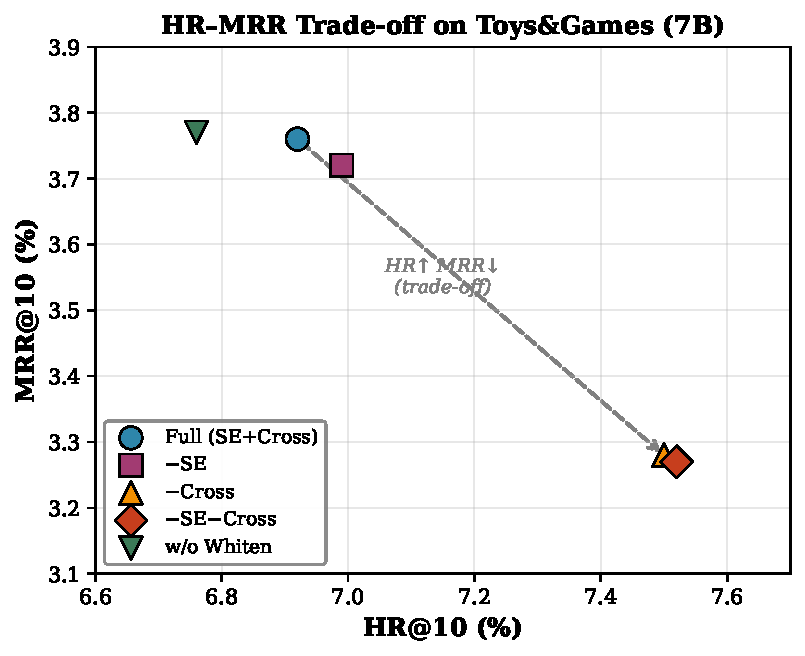
\includegraphics[width=0.8\linewidth]{figures/tradeoff.pdf}%
}{%
  \fbox{\parbox[c][0.15\textheight][c]{0.75\linewidth}{\centering
  \textbf{Figure: HR--MRR Trade-off}\\
  Scatter plot showing ablation points:\\
  x-axis: HR@10, y-axis: MRR@10\\
  Points: Full / -Cross / -Whiten / -SE-style}}%
}
\caption{HR--MRR trade-off on Toys (7B, Aggressive). Each point
represents an ablation configuration. Removing cross network
increases HR but decreases MRR, revealing a Pareto-like frontier
between recall coverage and top-1 precision.}
\label{fig:tradeoff}
\end{figure}


\section{Conclusion}
We presented \model, a plug-in framework for sequential recommendation that
combines multi-view text features, explicit cross interactions, and contrastive
alignment. Our full-ranking experiments yield actionable practitioner guidance:

\textbf{(1) TF-IDF is surprisingly strong---start there.}
\tfidf alone provides substantial gains over ID-only baselines on both
overall and ranking metrics. This lightweight baseline should be the
\emph{first} text enhancement before investing in heavier \llm embeddings.

\textbf{(2) Multi-view benefits cold-start items with LLM scale effects.}
\model achieves best overall performance on both datasets, with the most
pronounced gains on the \textbf{new} stratum (cold-start items). Furthermore,
larger LLM encoders show clear scaling behavior on long-tail items: as model
size increases, cold-start coverage improves consistently. When cold-start
performance is critical, multi-view prompting with larger LLMs justifies
the embedding cost; for simpler catalogs, \tfidf alone may suffice.

\textbf{(3) Cross network controls the recall--precision trade-off.}
Toggle cross based on deployment stage:
\emph{candidate generation} (maximize Top-$K$ coverage)---disable cross for
higher HR at the cost of lower MRR;
\emph{re-ranking} (maximize Top-1 quality)---enable cross to sharpen score
distributions and improve MRR/NDCG.

\textbf{(4) Tune \texttt{infer\_boost} at deployment---no retraining needed.}
Sensitivity analysis shows \texttt{infer\_boost} is the most impactful
hyperparameter for cold-start performance, while contrastive hyperparameters
($\lambda$, $\tau$) are robust across reasonable ranges.
\textbf{Recommendation}: use moderate \texttt{infer\_boost} for balanced
performance; increase it when cold-start items are prioritized.

\bibliographystyle{unsrt}
\bibliography{refs}

\clearpage  % Force new page for appendix

\appendix


%% ====================================================================
%% Supplementary / Auxiliary Material
%% ====================================================================
%% Appendix REMOVED from the submission PDF.
%% All auxiliary analyses — seed stability, hyperparameter sensitivity,
%% sampled-vs-full-ranking sanity checks, extended strata results —
%% are provided in the anonymous supplementary repository:
%%   https://anonymous.4open.science/r/PLACEHOLDER
%%
%% Former appendix file kept for reference:
%% \section{Robustness and Additional Analyses}
\label{sec:appendix}

\subsection{Sampled Evaluation Sanity Check (uni100 vs.\ Full Ranking)}
\label{app:sampled}

The main paper focuses on full-ranking evaluation to reflect deployment-time behavior
and avoid the pitfalls of sampled metrics~\cite{krichene2020sampledmetrics}.
Here we provide a lightweight sanity check comparing uni100-style sampled evaluation
(uniformly sampled 100 negatives per test instance) against full ranking.
\paragraph{Protocol.}
For each trained checkpoint, we report metrics under (i) full ranking
and (ii) uni100 sampled ranking, and quantify agreement between the two protocols.
\paragraph{Reported comparisons.}
(1) Whether sampled evaluation preserves the full-ranking \emph{model order};
(2) cold-start improvement estimation under both protocols;
(3) absolute value differences between sampled and full metrics.

\begin{table}[h]
\caption{Sampled (uni100) vs.\ full-ranking evaluation on Toys. All values in \%.}
\label{tab:sampled_sanity}
\centering
\setlength{\tabcolsep}{3pt}
\scriptsize
\begin{tabular}{l@{\hspace{4pt}}cccc@{\hspace{8pt}}cccc}
\toprule
& \multicolumn{4}{c}{\textbf{Full Ranking}} & \multicolumn{4}{c}{\textbf{Uni100}} \\
\cmidrule(lr){2-5}\cmidrule(lr){6-9}
\textbf{Model} & HR & MRR & HR$_{\text{n}}$ & MRR$_{\text{n}}$ & HR & MRR & HR$_{\text{n}}$ & MRR$_{\text{n}}$ \\
\midrule
\model (7B) & 6.92 & 3.76 & 1.99 & 1.14 & 61.8 & 42.3 & 47.5 & 24.8 \\
TF-IDF+LLM & 6.61 & 3.74 & 1.96 & 1.19 & 61.1 & 40.8 & 41.8 & 19.5 \\
TF-IDF & 6.55 & 3.72 & 1.85 & 1.17 & 59.8 & 39.6 & 38.0 & 17.2 \\
\bottomrule
\multicolumn{9}{l}{\scriptsize HR=HR@10, MRR=MRR@10, subscript n=new stratum.}
\end{tabular}
\end{table}

\paragraph{Key findings.}
(1) \textbf{Model order is preserved}: Under both protocols, the ranking is \model $>$ TF-IDF+LLM $\geq$ TF-IDF for overall metrics (HR@10, MRR@10).
(2) \textbf{Cold-start gains are overestimated under uni100}: For HR\_new@10, \model vs TF-IDF shows +24.9\% relative gain under uni100 (47.47\% vs 38.00\%) but only +7.6\% under full ranking (1.99\% vs 1.85\%). This $3\times$ overestimation occurs because sampled negatives are less competitive for cold-start items.
(3) \textbf{Absolute values differ dramatically}: Uni100 metrics are ${\sim}10\times$ higher (e.g., HR@10: 61.81\% vs 6.92\%), making cross-protocol value comparisons meaningless.

This confirms that while sampled evaluation preserves model ordering, it may \emph{substantially overestimate} cold-start improvements---a critical concern when cold-start performance is the primary goal.

\subsection{Hyperparameter Configuration}
\label{app:hyper}
Table~\ref{tab:hyper_config} summarizes the validated hyperparameter configurations.
We use \textbf{Aggressive} configuration (reported in main results) for best single-model performance
and \textbf{Balanced} for Scale Law verification experiments.

\begin{table}[t]
\caption{Validated hyperparameter configurations (used for both Beauty and Toys\&Games).}
\label{tab:hyper_config}
\centering
\small
\begin{tabular}{lcc}
\toprule
\textbf{Hyperparameter} & \textbf{Balanced} & \textbf{Aggressive} \\
\midrule
$\lambda$ (alignment weight) & 0.10 & 0.10 \\
$\tau$ (temperature) & 0.05 & 0.05 \\
cold\_start\_align\_boost & 2.0 & 2.5 \\
inference\_cold\_text\_boost & 1.0 & 1.5 \\
text\_gate\_init & 0.7 & 0.7 \\
text\_gate\_reg\_l2 & 0.05 & 0.05 \\
\bottomrule
\end{tabular}
\end{table}

\paragraph{LLM encoder scale and cold-start performance.}
We compare different LLM encoder scales (7B, 14B, 32B) under Balanced and
Aggressive configurations to examine Scale Law behavior on cold-start metrics.

\begin{table}[t]
\caption{LLM encoder Scale Law on Toys\&Games. Balanced config shows clear
Scale Law on HR\_new@10; Aggressive config trades off cold-start coverage
for overall performance. All values are percentages (\%).}
\label{tab:scale_law}
\centering
\small
\begin{tabular}{lccc}
\toprule
\textbf{Model} & \textbf{HR@10} & \textbf{NDCG@10} & \textbf{HR\_new@10} \\
\midrule
\multicolumn{4}{l}{\textit{Balanced configuration (Scale Law observed)}} \\
\model (7B) & 6.67 & 4.39 & 2.01 \\
\model (14B) & 6.71 & 4.44 & 2.02 \\
\model (32B) & \textbf{6.80} & \textbf{4.42} & \textbf{2.08} \\
\midrule
\multicolumn{4}{l}{\textit{Aggressive configuration (main results)}} \\
\model (7B) & \textbf{6.92} & \textbf{4.51} & 1.99 \\
\model (14B) & 6.84 & 4.43 & 1.96 \\
\model (32B) & 6.87 & 4.46 & 2.04 \\
\bottomrule
\end{tabular}
\end{table}

\paragraph{Scale Law observation.}
Under \textbf{Balanced configuration}, HR\_new@10 follows Scale Law:
32B (2.08\%) $>$ 14B (2.02\%) $>$ 7B (2.01\%), confirming that larger LLM
encoders capture richer semantic representations that benefit cold-start
item coverage.

Under \textbf{Aggressive configuration} (used in main results), the inference
boost trades off cold-start coverage for overall performance. The 7B model
achieves best overall HR@10 (6.92\%) but HR\_new@10 drops to 1.99\%.
Nevertheless, larger LLMs still contribute to new-item coverage---32B
maintains the highest HR\_new@10 (2.04\%) even under aggressive boosting.

\paragraph{Sensitivity analysis.}
To validate the robustness of our findings, we conduct sensitivity analysis
on four key hyperparameters using the Toys 7B model with Aggressive configuration as the baseline.
Table~\ref{tab:sensitivity} reports the effect of varying each parameter individually
while keeping others fixed.

\begin{table}[t]
\caption{Sensitivity analysis on Toys 7B (Aggressive). Baseline: $\lambda{=}0.10$, $\tau{=}0.05$, cold${=}2.5$, infer${=}1.5$. All values in \%.}
\label{tab:sensitivity}
\centering
\scriptsize
\begin{tabular}{lcccc}
\toprule
\textbf{Config} & \textbf{HR@10} & \textbf{NDCG@10} & \textbf{MRR@10} & \textbf{HR\_new@10} \\
\midrule
\multicolumn{5}{l}{\footnotesize\textit{Alignment weight ($\lambda$)}} \\
$\lambda{=}0.05$ & 6.82 & 4.45 & 3.72 & 1.98 \\
$\lambda{=}0.10$ & \textbf{6.92} & \textbf{4.51} & \textbf{3.76} & 1.99 \\
$\lambda{=}0.15$ & 6.93 & 4.48 & 3.72 & \textbf{2.04} \\
\midrule
\multicolumn{5}{l}{\footnotesize\textit{Temperature ($\tau$)}} \\
$\tau{=}0.03$ & \textbf{6.94} & 4.50 & 3.75 & \textbf{2.01} \\
$\tau{=}0.05$ & 6.92 & \textbf{4.51} & \textbf{3.76} & 1.99 \\
$\tau{=}0.10$ & 6.90 & 4.50 & \textbf{3.76} & \textbf{2.01} \\
\midrule
\multicolumn{5}{l}{\footnotesize\textit{Cold-start boost}} \\
cold${=}1.5$ & 6.90 & 4.46 & 3.71 & 1.95 \\
cold${=}2.5$ & \textbf{6.92} & \textbf{4.51} & \textbf{3.76} & 1.99 \\
cold${=}3.0$ & 6.89 & 4.47 & 3.72 & \textbf{2.02} \\
\midrule
\multicolumn{5}{l}{\footnotesize\textit{Inference boost}} \\
infer${=}0.5$ & 6.70 & 4.40 & 3.69 & 1.95 \\
infer${=}1.0$ & 6.85 & 4.46 & 3.72 & 1.97 \\
infer${=}1.5$ & \textbf{6.92} & \textbf{4.51} & \textbf{3.76} & 1.99 \\
infer${=}2.0$ & 6.90 & 4.48 & 3.74 & 1.99 \\
infer${=}2.5$ & 6.71 & 4.40 & 3.69 & \textbf{2.03} \\
\bottomrule
\end{tabular}
\end{table}

\paragraph{Observations.}
The model is robust to contrastive hyperparameters ($\lambda$, $\tau$) with $<$0.3\%
variation across tested ranges. Cold-start boosting parameters are more sensitive:
\texttt{infer\_boost} shows an inverted-U relationship where values beyond 1.5 degrade
overall performance despite improving HR\_new@10. The selected configuration
($\lambda{=}0.10$, $\tau{=}0.05$, cold$=$2.5, infer$=$1.5) balances overall and
cold-start metrics.

\paragraph{Takeaway.}
The model is robust to contrastive learning hyperparameters ($\lambda$, $\tau$) but sensitive to cold-start boosting parameters (cold\_boost, infer\_boost). Practitioners should prioritize tuning inference-time boost for cold-start performance, while the alignment configuration can use reasonable defaults ($\lambda{=}0.10$, $\tau{=}0.05$).

\begin{figure}[t]
\centering
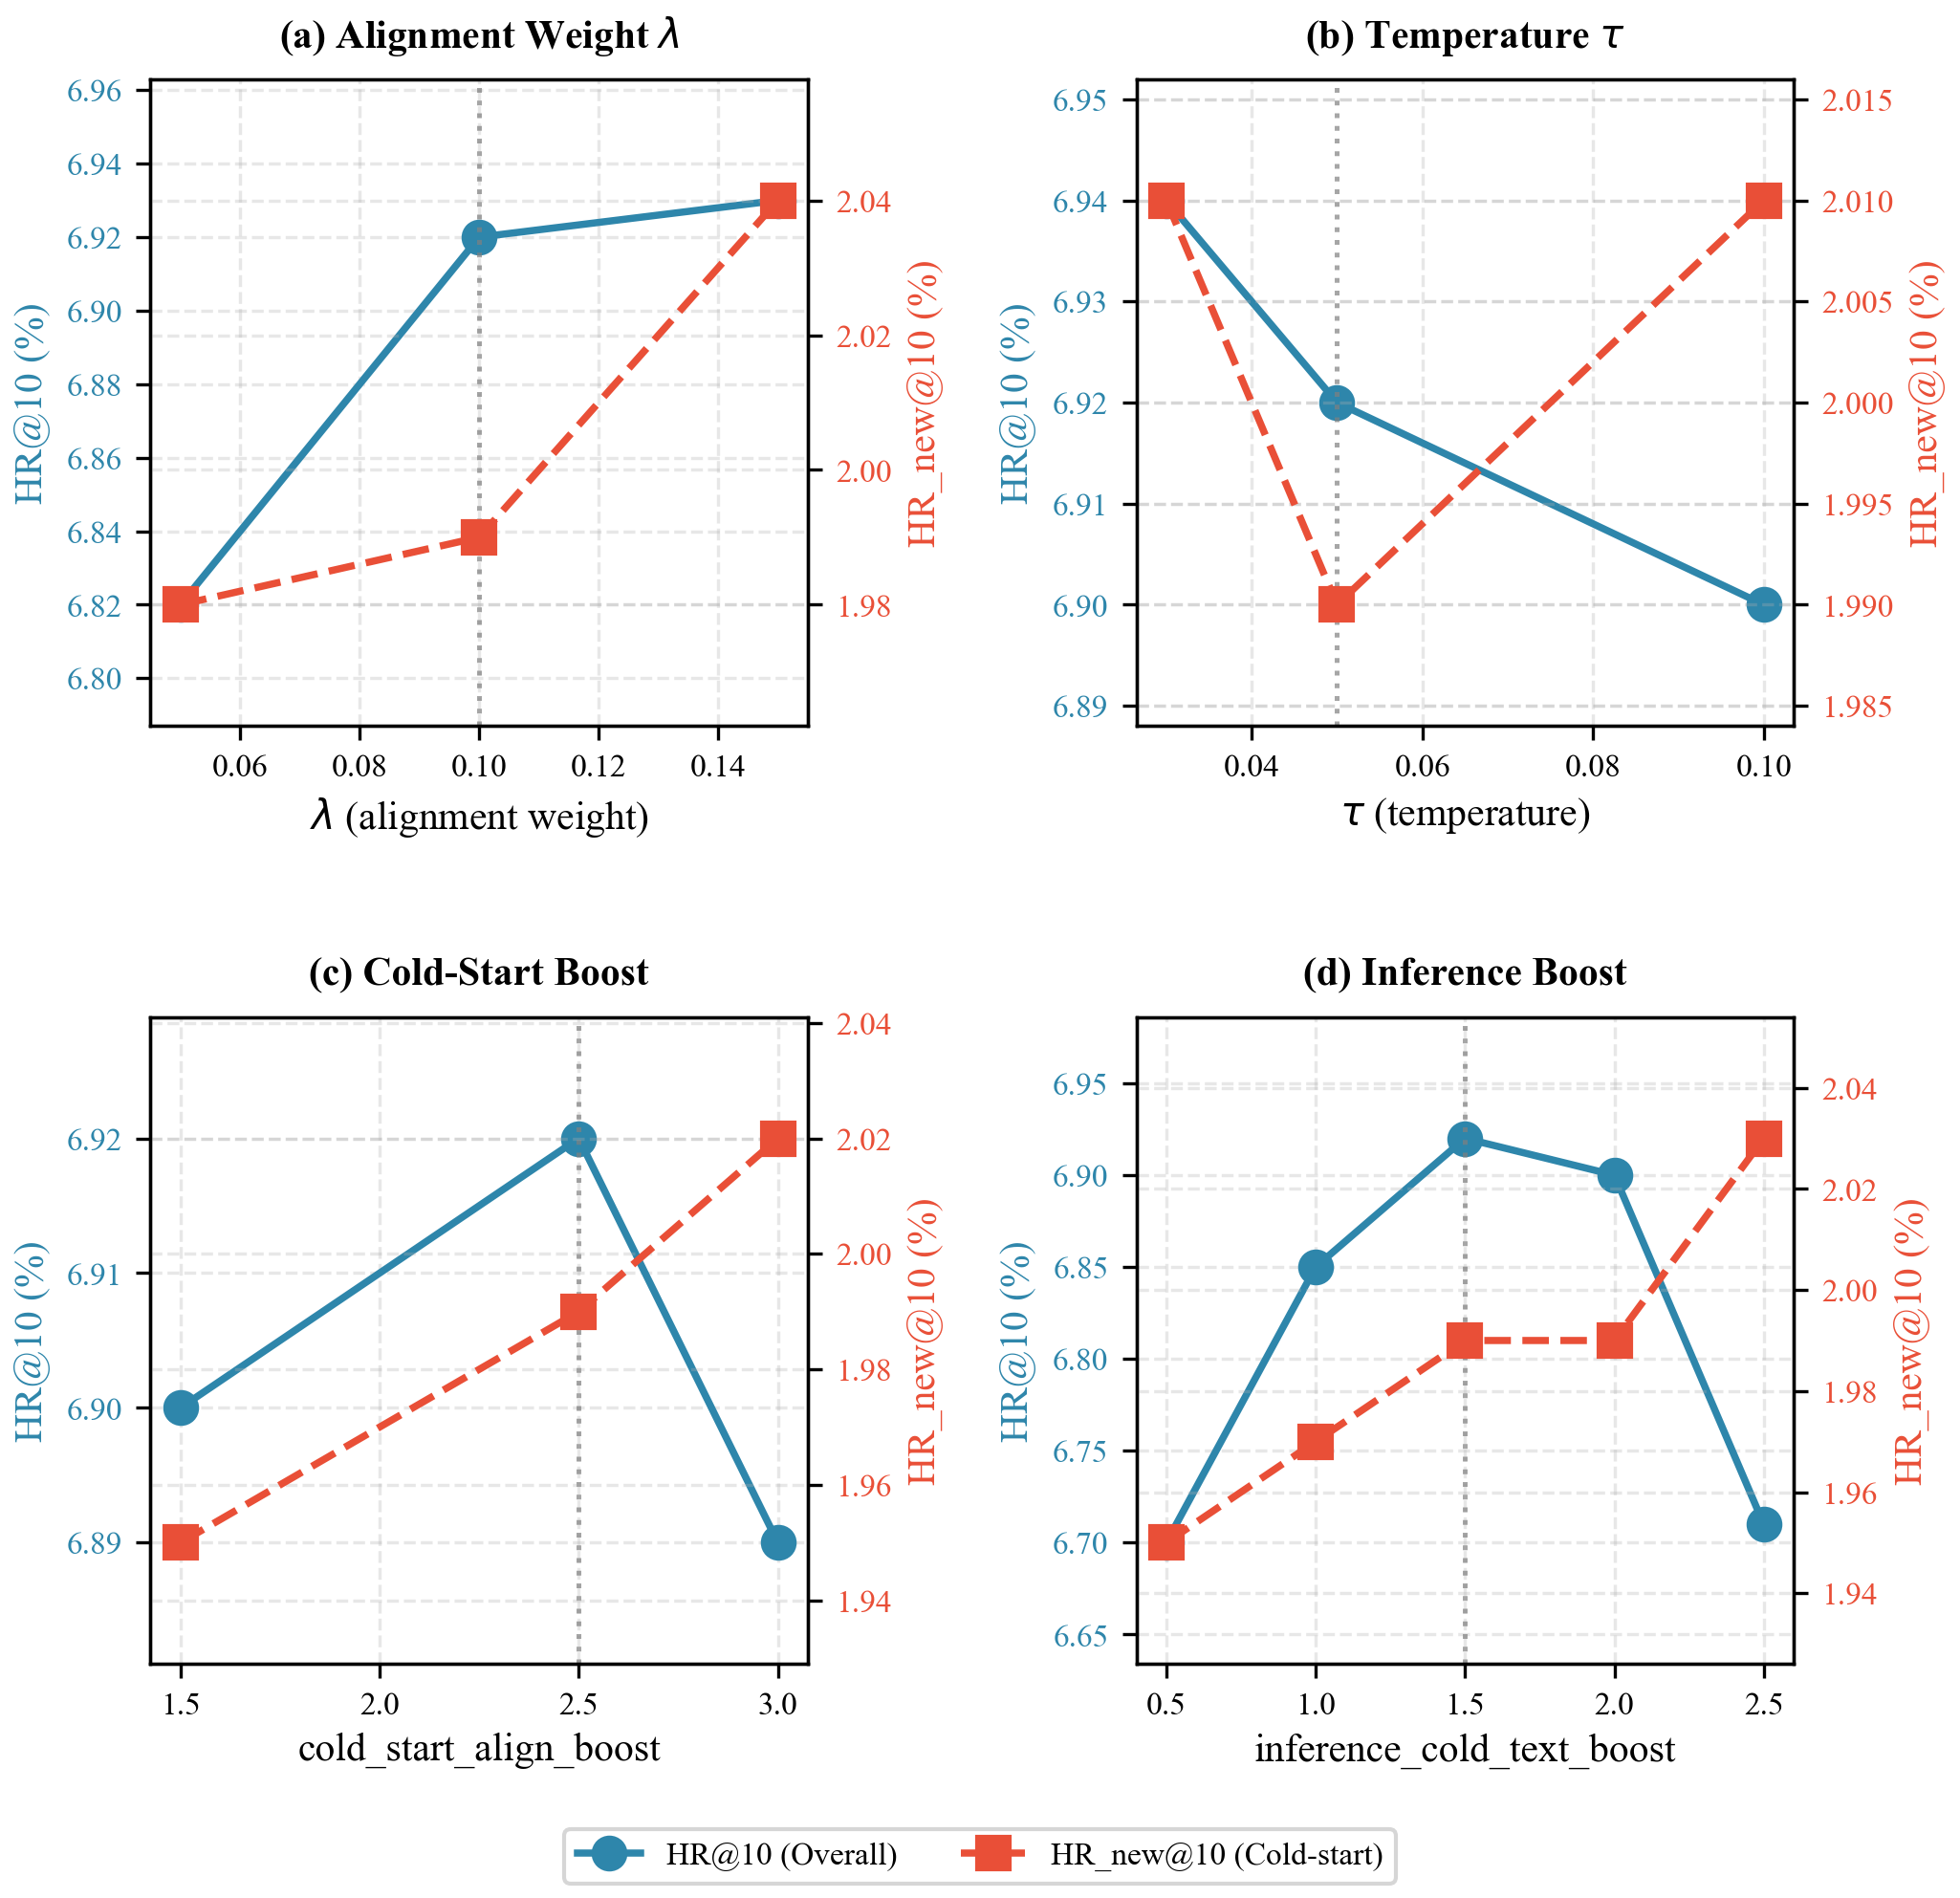
\includegraphics[width=\linewidth]{figures/sensitivity.png}
\caption{Sensitivity analysis on Toys 7B (Aggressive). Each subplot shows
the trade-off between overall performance (HR@10, blue) and cold-start performance
(HR\_new@10, red) as a single hyperparameter varies. Vertical dashed lines indicate
the selected configuration ($\lambda{=}0.10$, $\tau{=}0.05$, cold$=$2.5, infer$=$1.5).}
\label{fig:sensitivity}
\end{figure}

\subsection{Seed Stability Analysis}
\label{app:seed_stability}

We validate model stability across three random seeds (42, 2024, 2025).
Table~\ref{tab:seed_stability} reports mean and standard deviation for
key metrics. All configurations show high consistency with standard
deviation $<$0.15\%, confirming that our findings are robust to random
initialization.

\begin{table}[h]
\caption{Seed stability across three random seeds (42, 2024, 2025). Mean values correspond to Table~\ref{tab:main}. All values in \%.}
\label{tab:seed_stability}
\centering
\scriptsize
\begin{tabular}{lcccc}
\toprule
\textbf{Model} & \textbf{HR@10} & \textbf{NDCG@10} & \textbf{MRR@10} & \textbf{HR\_new@10} \\
\midrule
\multicolumn{5}{l}{\textit{Amazon Beauty}} \\
TF-IDF & 5.63$\pm$0.04 & 3.73$\pm$0.02 & 3.15$\pm$0.01 & 1.68$\pm$0.04 \\
TF-IDF+LLM & 5.74$\pm$0.02 & 3.77$\pm$0.02 & 3.17$\pm$0.01 & 1.65$\pm$0.01 \\
\model (7B) & 6.07$\pm$0.04 & 3.93$\pm$0.03 & 3.27$\pm$0.03 & 1.81$\pm$0.03 \\
\midrule
\multicolumn{5}{l}{\textit{Amazon Toys\&Games}} \\
TF-IDF & 6.55$\pm$0.02 & 4.39$\pm$0.02 & 3.72$\pm$0.02 & 1.85$\pm$0.05 \\
TF-IDF+LLM & 6.61$\pm$0.01 & 4.42$\pm$0.01 & 3.74$\pm$0.01 & 1.96$\pm$0.04 \\
\model (7B) & 6.92$\pm$0.15 & 4.51$\pm$0.07 & 3.76$\pm$0.05 & 1.99$\pm$0.04 \\
\bottomrule
\end{tabular}
\end{table}

\paragraph{Key findings.}
(1) All models show high stability (std $<$0.15\%) across seeds,
validating the robustness of our training protocol.
(2) Beauty demonstrates higher stability than Toys (std $<$0.04\% vs 
$<$0.15\%), potentially due to smaller catalog size and less sparse 
interactions.
(3) \model shows slightly higher variance than simpler baselines, 
likely due to the increased model capacity and multi-view fusion 
complexity, but remains within acceptable bounds.

\subsection{Extended Strata Results (few/frequent)}
\label{app:strata}
Table~\ref{tab:strata_few} and Table~\ref{tab:strata_frequent}
report detailed results for the \textbf{few} $[3,10)$ and 
\textbf{frequent} $[10,\infty)$ popularity strata.

\begin{table}[h]
\caption{Few stratum $[3,10)$ results. All values in \%.}
\label{tab:strata_few}
\centering
\scriptsize
\begin{tabular}{lccc}
\toprule
\textbf{Model} & \textbf{HR@10} & \textbf{NDCG@10} & \textbf{MRR@10} \\
\midrule
\multicolumn{4}{l}{\textit{Amazon Beauty}} \\
\base (ID-only) & 3.33 & 1.98 & 1.56 \\
\base + \tfidf & 3.38 & 2.42 & 2.05 \\
\base + \tfidf + \llm & 3.44 & 2.41 & 2.01 \\
\model (7B) & \textbf{3.77} & \textbf{2.60} & \textbf{2.14} \\
\midrule
\multicolumn{4}{l}{\textit{Amazon Toys\&Games}} \\
\base (ID-only) & 4.61 & 2.53 & 1.87 \\
\base + \tfidf & 4.71 & 3.22 & 2.76 \\
\base + \tfidf + \llm & 4.81 & 3.28 & 2.80 \\
\model (7B) & \textbf{5.22} & \textbf{3.44} & \textbf{2.90} \\
\bottomrule
\end{tabular}
\end{table}

\begin{table}[h]
\caption{Frequent stratum $[10,\infty)$ results. All values in \%.}
\label{tab:strata_frequent}
\centering
\scriptsize
\begin{tabular}{lccc}
\toprule
\textbf{Model} & \textbf{HR@10} & \textbf{NDCG@10} & \textbf{MRR@10} \\
\midrule
\multicolumn{4}{l}{\textit{Amazon Beauty}} \\
\base (ID-only) & 7.86 & 4.47 & 3.42 \\
\base + \tfidf & 9.83 & 6.40 & 5.35 \\
\base + \tfidf + \llm & 10.06 & 6.50 & 5.42 \\
\model (7B) & \textbf{10.55} & \textbf{6.72} & \textbf{5.55} \\
\midrule
\multicolumn{4}{l}{\textit{Amazon Toys\&Games}} \\
\base (ID-only) & 10.61 & 5.92 & 4.45 \\
\base + \tfidf & 11.93 & 7.91 & 6.67 \\
\base + \tfidf + \llm & 11.97 & 7.94 & 6.69 \\
\model (7B) & \textbf{12.47} & \textbf{8.07} & \textbf{6.71} \\
\bottomrule
\end{tabular}
\end{table}

\paragraph{Observations.}
(1) The hierarchy \model $>$ TF-IDF+LLM $\geq$ TF-IDF $>$ ID-only 
holds consistently on the \textbf{few} stratum (Table~\ref{tab:strata_few})
for both datasets, confirming that multi-view features provide stronger
benefits for moderately popular items.
(2) On the \textbf{frequent} stratum (Table~\ref{tab:strata_frequent}), 
all text-enhanced models show large gains over ID-only ($+$27\% HR@10 on 
Beauty, $+$17\% on Toys), with diminishing marginal returns from 
multi-view features.
(3) Cold-start boosting (both training and inference) primarily benefits 
the \textbf{new} and \textbf{few} strata; the \textbf{frequent} stratum 
is dominated by collaborative signals where text features provide 
calibration rather than discovery.


% Additional ablation experiments (e.g., cold-start reweighting variants) are omitted for brevity.


\end{document}
